In the previous chapter, we have learned how an interpreted programming language can be implemented.
Another method of implementing a programming language is to create a compiler for this language.
However, the question of how such a compiler works exactly still remains.

\section{How a Compiler Translates the AST}

\begin{wrapfigure}{R}{0.52\textwidth}
	\centering
	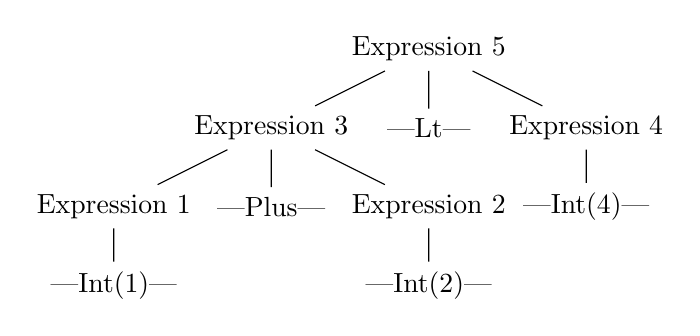
\begin{tikzpicture}[level distance=1cm, sibling distance=2cm]
		\node {Expression 5}
		child {node {Expression 3}
				child {node {Expression 1}
						child {node {\Verb|Int(1)|}}}
				child {node {\Verb|Plus|}}
				child {node {Expression 2}
						child {node {\Verb|Int(2)|}}}}
		child {node {\Verb|Lt|}}
		child {node {Expression 4}
				child {node {\Verb|Int(4)|}}};
	\end{tikzpicture}
	\caption{Abstract Syntax Tree for `\texttt{1+2 < 4}'}\label{fig:cmp_simple_tree}
\end{wrapfigure}

Often, a compiler traverses an AST generated by the analyzer in order to translate it to some sort of output.
For each AST node, the compiler usually calls a separate function or method which is specialized in translating this specific node type.
These individual functions often return some sort of value representing the translated node.
Otherwise, each individual function may also insert generated instructions into an internal field of the compiler.
Here, the newly generated instruction is inserted the output sequence of instructions.
In this case, each function often also returns metadata about the previously compiled node.
For instance, this data may include the register or memory location of a previously compiled expression, so that other AST nodes can refer to it later.
In transpilers, meaning compilers translating one high-level language into another one, each node-specific function often returns a tree node representing code in the output language.

Listing~\ref{fig:cmp_simple_tree} displays a simplified syntax tree of the rush expression `\texttt{1+2 < 4}'.
The number after each expression represents the order in which most compilers would traverse this tree.
Compilation of the expression starts at the root node of the tree.
Here, most compilers will begin translation by first compiling the child nodes using \emph{post-order} traversal.
Post-order traversal is frequently used because the compilation of a node often depends on the output of its child nodes.
In this example, translation of the root comparison expression depends on the information returned by compiling its left- and right-hand sides.
Therefore, the compiler first considers the node `Expression 3' which represents the add-expression \texttt{1+2}.
However, due to post-order traversal, this node is not actually traversed since the compiler skips straight to its child nodes.
Therefore, the left child `Expression 1' is traversed as the very first node.
Next, its sibling node `Expression 4' is traversed too.
Since post-order traversal involves considering a root node after the traversal of its children, `Expression 3' is traversed after its children have been considered.
Here, the compiler considers the operand of the expression in order to generate the appropriate output instruction.
Therefore, the instruction responsible for the addition is inserted after the Expression node 3 has been traversed.
Since `Expression 3' and its children are now completely traversed, and its output instruction has been inserted, the compiler now considered the right-hand side of the comparison.
Here, the node `Expression 2' only consists of the constant integer value 4.
Now, all child nodes of `Expression 5' have been traversed, thus the compiler now considers this node itself.
Here, the compiler notices that the expression should check if the left-hand side is less than the right-hand side.
Therefore, the compiler inserts an instruction performing this comparison using the results of the left and right child as the operands.
Since the compiler must be aware of the operands of the instruction, each method or function involved in the tree-traversal returns an entity describing the location of the runtime value of its previously compiled node.
For instance, if the target architecture uses registers, every method translating an expression must return the register containing the value of the expression at runtime.
Therefore, such a describing entity can either be a register or a memory location describing the location a value which a node may yield.
By returning information like this, a root node will have information about its children after they have been traversed.
A root node might rely on the values returned by its children, therefore it is traversed at last, thus creating the demand for post-order traversal.

\Lirsting[raw=true, caption={Simple Pseudo-Instructions For a Fictional Architecture}, label={lst:cmp_simple_instructions}, float=H]{listings/simple_compiler_instructions.txt}

Listing~\ref{lst:cmp_simple_instructions} displays a sequence of instructions for a fictional architecture.
This sequence could have been generated from the previously discussed tree in Figure~\ref{fig:cmp_simple_tree}.
It is apparent that the order of instructions matches the order in which the tree was traversed.
The instructions in line 1 and 2 represent the tree-nodes `Expression 1' and `Expression 2' respectively.
Here, the value 1 is assigned to a register named `\texttt{r0}' whilst the value 2 is assigned to the register `\texttt{r1}'.
The \texttt{add} instruction in line 3 appears after the instructions in line 1 and 2 since their tree nodes were traversed first.
Furthermore, the instruction uses register \texttt{r0} and \texttt{r1} as its operands and therefore depends on them containing a value.
Therefore, the \texttt{add} instruction can use the registers returned by compiling its child nodes as its operands.
Next, the constant integer value 4 is assigned to the register `\texttt{r3}'.
Lastly, the comparison instruction `lt' is inserted using the result of the addition and the register containing 4 as its operands.
Here, it is apparent that the instruction generated by the node which was traversed at last is also inserted at the end.

Therefore, using post-order traversal in order to generate output instructions targeting a register-based architecture is often required.
This example illustrates how a simple compiler might operate.
However, a similar algorithm is often found in even the most complex compilers.
